\chapter{Probability Rules}
\section{General Rules}
Here are a few basic rules of probabilities. They should be relatively straightforward.
\begin{theorem}
For a sample space, \sS, the probability of a simple event in \sS~occurring is 1. That is
\[
    P(\sS) = 1
\]
\end{theorem}
\begin{proof}
\[
    P(\sS) = \sum_{a \in \sS} P(a) = \sum_{\all a} P(a)
\]
\end{proof}
\begin{theorem}
Any event $A$ in a sample space has a probability between 0 and 1 inclusive. That is
\[
    0 \leq P(A) \leq 1 \for\all A\subseteq\sS
\]
\end{theorem}
\begin{proof}
Note that $A$ is a subset of \sS, so
\[
    P(A) = \sum_{a \in A} P(a) \leq \sum_{a \in \sS} P(a) = 1
\]
Now, recall that $P(a) \geq 0$ for any sample point $a$ by our probability model. Thus, since $P(A)$ is the sum of non-negative real numbers, $P(A) \geq 0$. So we have
\[
    1 \leq P(A) \leq 1
\]
\end{proof}
\begin{theorem}
If $A$ and $B$ are two events such that $A \subseteq B$, that is all the sample points in $A$ are also in $B$, then 
\[
    P(A) \leq P(B)
\]
\end{theorem}
\begin{proof}
\[
    P(A) = \sum_{a \in A} P(a) \leq \sum_{a \in B} P(a) = P(B)
\]
\end{proof}
% ------------------------------------------------- %
\section{Venn Diagrams}
As we have seen already, it is helpful to think of events in a sample space as subsets of the sample space. Consider a sample space, $\sS = \{\, 1,2,3,4,5,6 \,\}$. A number is picked at random, let $E$ be the event that the number is even. We can think of $E$ as the subsets of \sS, $\{\, 2,4,6 \,\}$ and the probability of $E$ is the probability of any sample points in $A$ occurs, that is 2, 4, or 6 is selected. We can represent the relationships of events in the sample space using Venn diagrams.
\par\smallskip
\begin{figure}[h]
\centering
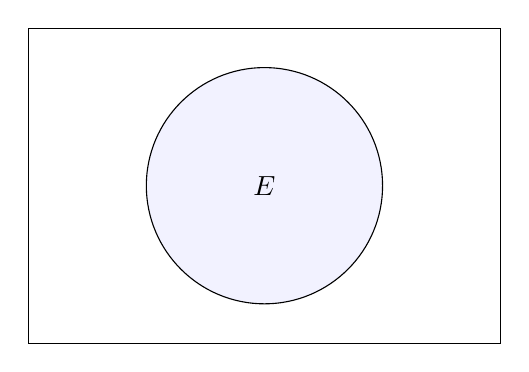
\begin{tikzpicture}
\draw (0,0) rectangle (6,4) node[below left] {$\sS$};
\filldraw[fill=blue!5] (3,2) circle (1.5) node {$E$};
\end{tikzpicture}
\caption{Single event $E$} \label{fig:Single event}
\end{figure}
Now, assuming the area of $E$ is half the area of \sS, we have that the probability of $E$ is the probability that a randomly chosen point on the area of \sS~will be within $E$.

Consider now we let $G = \{\, 4,5,6 \,\}$ be the event that that the number selected is greater than or equal to 4. We have
\par\smallskip
\begin{figure}[h]
\centering
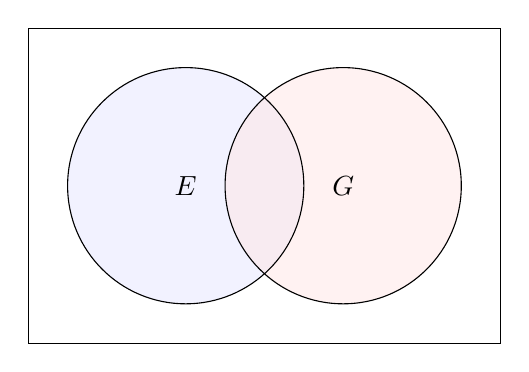
\begin{tikzpicture}

\def\eventE{(2,2) circle (1.5)}
\def\eventG{(4,2) circle (1.5)}

\draw (0,0) rectangle (6,4) node[below left] {$\sS$};

\begin{scope}[fill opacity=0.5]
\fill[blue!10] \eventE;
\fill[red!10] \eventG;
\end{scope}

\draw \eventE node {$E$};
\draw \eventG node {$G$};

\end{tikzpicture}
\caption{Events $E$ and $G$} \label{fig:Events E and G}
\end{figure}
The total shaded region of the Venn diagram, $E \union G$, contains all the sample points of $E$ and $G$. It is the event that any outcome in either $E$ or~$G$, or both, occurs. Thus, $E \union G$ is the event that $E$, $G$ or~both, occurs. Similarly, the union of three events is the event that at least one of the three events occur.

Consider now the intersection $E \intersect G$. It is the set of all the points that are in both $E$ and~$G$, $\{\, 4,6 \,\}$. Thus, it is the event that an outcome in both $E$ and $G$ occurs. So $E \intersect G$ is the event that $E$ and~$G$ both occur. 
\begin{info}
The sets $A \intersect B$ and similarly $A \intersect B \intersect C$ are often denoted as $AB$ and $ABC$ respectively.
\end{info}
Finally, the unshaded space in Figure 4.1 is the set of all outcomes that are not in~$E$. It is the complement of $E$ and is denoted by $\comp{E}$. It is the event that $E$ does not occur.
\begin{info}
Note that the complement of \sS~is the null set, that is $\comp{\sS} = \nullset$, and has a probability of 0.
\end{info}
% ------------------------------------------------- %
\section{De Morgan's Laws}
\begin{theorem}
The following are De Morgan's Laws:
\begin{enumerate}
    \item $\comp{A \union B} = \comp{A} \intersect \comp{B}$
    \item $\comp{A \intersect B} = \comp{A} \union \comp{B}$
\end{enumerate}
\end{theorem}
% Include a proof here #;target
\section{Rules for Unions of Events}
Recall Figure 4.2, copied below.
\par
\begin{figure}[h]
\centering
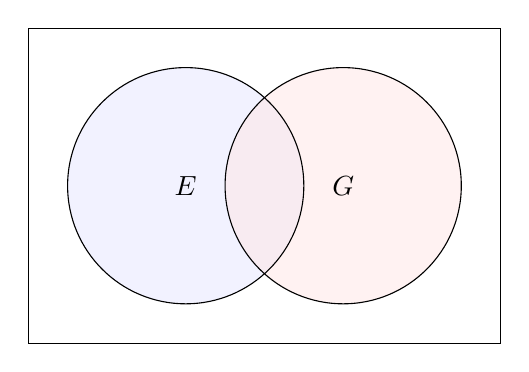
\begin{tikzpicture}

\def\eventE{(2,2) circle (1.5)}
\def\eventG{(4,2) circle (1.5)}

\draw (0,0) rectangle (6,4) node[below left] {$\sS$};

\begin{scope}[fill opacity=0.5]
\fill[blue!10] \eventE;
\fill[red!10] \eventG;
\end{scope}

\draw \eventE node {$E$};
\draw \eventG node {$G$};

\end{tikzpicture}
\repeatcaption{fig:Events E and G}{Events E and G}
\end{figure}
We can see that the area of $E \union G$ is not simply the sum of the areas of $E$ and~$G$. So we have that the probability of $E \union G$ is not simply the sum of the probability of $E$ and $G$. Rather, we must sum the probabilities and subtract the intersection (which gets included twice in the sum) to obtain $P(E \union G)$.
\begin{theorem}
For any events, $A$ and $B$, in a sample space, we have
\[
    P(A \union B) = P(A) + P(B) - P(A \intersect B)
\]
\end{theorem}
\begin{example}
A number between 1 and 6 inclusive is chosen randomly. Let $E = \{\, 2,4,6 \,\}$ be the event the number is odd and let $G = \{\, 4,5,6 \,\}$ be the event that the number is greater than or equal to 4.
\par\smallskip
The probability of the number being even \textbf{or} greater than 4 is $P(E \union G)$. Since both $E$ and~$G$ contain 3~points of the six in the sample space, $P(E) = P(G) = 1/2$. Thus, we can see clearly that $P(E \union G) \neq P(E) + P(G) = 1$ since $\{\, 1 \,\}$ is not in $E$ or $G$ and has a probability of 1/6. Now, note $E \intersect G = \{\, 4,6 \,\}$, so $P(E \intersect G) = 1/3$. We have
\[
    P(E \union G) = P(E) + P(G) - P(E \intersect G) = 1/2 + 1/2 - 1/3 = 2/3
\]
\end{example}
\pagebreak[3]
Now consider the case of the union of three events.\par
\begin{figure}[ht]
\centering
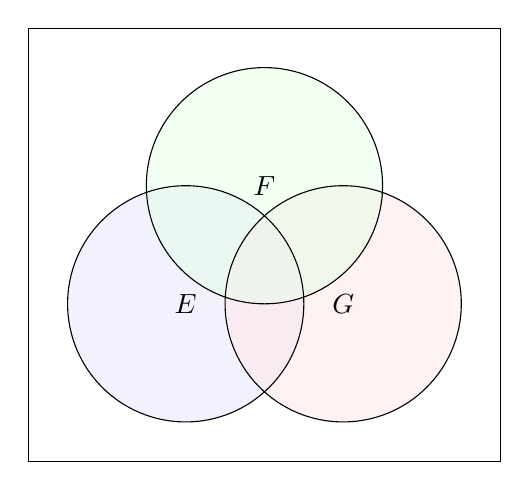
\begin{tikzpicture}

\def\eventE{(2,2) circle (1.5)}
\def\eventG{(4,2) circle (1.5)}
\def\eventF{(3,3.5) circle (1.5)}

\draw (0,0) rectangle (6,5.5) node[below left] {$\sS$};

\begin{scope}[fill opacity=0.5]
\fill[blue!10] \eventE;
\fill[red!10] \eventG;
\fill[green!10] \eventF;
\end{scope}

\draw \eventE node {$E$};
\draw \eventG node {$G$};
\draw \eventF node {$F$};

\end{tikzpicture}
\caption{Three events} \label{fig:Three events}
\end{figure}
Let $A_I$ be the area on the Venn diagram of the event $I$. The area of the union once again is not simply the sum of the areas ($A_E + A_G + A_F$). Instead we can reason out that when we add the three areas we include $A_{E \intersect G}$, $A_{G \intersect F}$, and $A_{F \intersect E}$ twice each and $A_{E \intersect G \intersect F}$ three times. The sum of these doubly counted areas ($A_{E \intersect G} + A_{G \intersect F} + A_{F \intersect E}$) also includes $A_{E \intersect G \intersect F}$ three times. Thus, when we subtract the area of the doubly counted segments, $A_{E \intersect G \intersect F}$ is also subtracted three times leaving this area unaccounted for. Therefore we then add $A_{E \intersect G \intersect F}$ to find the complete area of $E \union G \union F$.
\begin{theorem}
For any events, $A$, $B$ and $C$, in a sample space, we have
\[
    P(A \union B \union C) = P(A) + P(B) + P(C) - P(A \intersect B) - P(B \intersect C) - P(C \intersect A) + P(A \intersect B \intersect C)
\]
\end{theorem}
\section{Mutually Exclusive Events}
Events $A$ and $B$ are mutually exclusive if and only if $A \intersect B = \nullset$. More simply, the events $A$ and $B$ cannot both occur in one experiment because they share no points in common and only one sample point is achieved.
\par\smallskip
In general, events $A_1,A_2,A_3,\ldots,A_n$ are mutually exclusive if and only if $A_i \intersect A_j = \nullset \for\all i \neq j$. This means that at most one of these events may occur in any one experiment.
\subsection*{Probability of the Unions of Mutually Exclusive Events}
Consider the Venn diagram of two mutually exclusive events, $E$ and $G$.
\begin{figure}[htp]
\centering
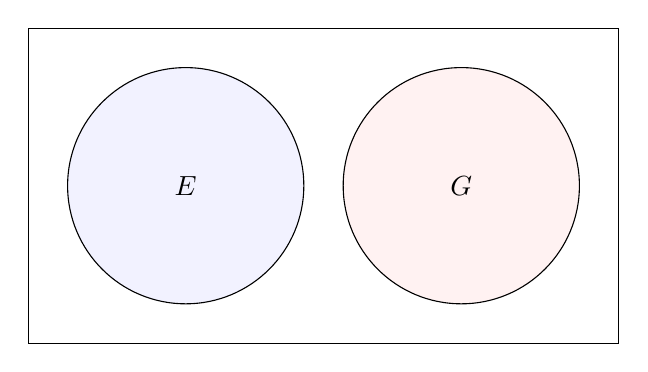
\begin{tikzpicture}

\def\eventE{(2,2) circle (1.5)}
\def\eventG{(5.5,2) circle (1.5)}

\draw (0,0) rectangle (7.5,4) node[below left] {$\sS$};

\begin{scope}[fill opacity=0.5]
\fill[blue!10] \eventE;
\fill[red!10] \eventG;
\end{scope}

\draw \eventE node {$E$};
\draw \eventG node {$G$};

\end{tikzpicture}
\caption{Two mutually exclusive events} \label{fig:Two mutually exclusive events}
\end{figure}
Clearly the probability of the intersection of two mutually exclusive events is 0, since it doesn't contains any sample points. So we have 
\[
    P(E \intersect G) = 0    
\]
Another intrinsic property of mutually exclusive events that we can see on a Venn diagram is that the area of $E \union G$ is the sum of the areas of $E$ and $G$. Therefore, unlike in previous examples, the probability of $E \union G$ is the sum of the probabilities of $E$ and $G$.
\begin{theorem}
For mutually exclusve events, $A$ and $B$, in a sample space, we have
\[
    P(A \union B) = P(A) + P(B)
\]
\end{theorem}
\begin{theorem}
More generally for $n$ mutually exclusive events, $A_1,A_2,\ldots,A_n$, in a sample space, we have
\[
    P(A_1 \union A_2 \union \cdots \union A_n) = P(A_1) + P(A_2) + \cdots + P(A_n) = \sum_{i = 1}^{n} P(A_i)
\]
\end{theorem}
\subsection*{Probabilities of Complements}
\begin{theorem}
For any event $A$, we have
\[
    P(A) = 1 - P(\comp{A})
\]
\end{theorem}
\begin{proof}
Recall the complement of an event consists of all the sample points not in the event. Thus, for any event~$A$, its complement~$\comp{A}$ contains no points in common with~$A$. So $A \intersect \comp{A} = \nullset$ and $A$ and~$\comp{A}$ are mutually exclusive, by~definition. Now, consider $A \union \comp{A}$, it spans the whole of the sample space so we have $P(A \union \comp{A}) = 1$ and since $A$ and $\comp{A}$ are mutually exclusive, we have
\[
    P(A) + P(\comp{A}) = 1
\]
and it follows that $P(A) = 1 - P(\comp{A})$, as required.
\end{proof}
\section{Independence of Events}
Events $A$ and $B$ are said to be independent if and only if $P(A \intersect B) = P(A)P(B)$. Otherwise they are dependent events.
\par\smallskip
In general, events $A_1,A_2,A_3\ldots,A_n$ are independent if and only if 
\[
    P(A_{i_1} \intersect A_{i_2} \intersect A_{i_3} \intersect \cdots \intersect A_{i_n}) = P(A_{i_1}) + P(A_{i_2}) + P(A_{i_3}) + \cdots + P(A_{i_n})
\]
for all sets $\{\, i_1,i_2,i_3,\ldots,i_k \,\}$ of distinct subscripts chosen from $\{\, 1,2,3,\ldots,n \,\}$.
\begin{example}
Consider an experiment in which a fair die is tossed twice. We define the following events:
\begin{itemize}[noitemsep, topsep=4pt plus 2pt minus 1pt]
    \item $A$: The first number rolled is a six
    \item $B$: The second number rolled is a six
    \item $C$: The sum of the numbers rolled is less than or equal to seven
    \item $D$: The sum of the numbers rolled is equal to seven
\end{itemize}
Suppose the event $A$ occurs. Does this have any impact on the probability of $B, C$ or $D$ occurring?
\par\smallskip
It is quite clear to see that the events $A$ and $B$ are independent events since rolling a six on the first toss has no impact on the number that will be rolled on the second toss. Now, events $B$ and $C$ from the onset appear to be dependent since if you roll a six on the first toss you must roll a one to make your total less than or equal to seven. To confirm this consider the sample space
\[
    \left\{
        \begin{array}{c@{,\ }c@{,\ }c@{,\ }c@{,\ }c@{,\ }c}
            (1,1) & (1,2) & (1,3) & (1,4) & (1,5) & (1,6) \\
            (2,1) & (2,2) & (2,3) & (2,4) & (2,5) & (2,6) \\
            (3,1) & (3,2) & (3,3) & (3,4) & (3,5) & (3,6) \\
            (4,1) & (4,2) & (4,3) & (4,4) & (4,5) & (4,6) \\
            (5,1) & (5,2) & (5,3) & (5,4) & (5,5) & (5,6) \\
            (6,1) & (6,2) & (6,3) & (6,4) & (6,5) & (6,6) \\
        \end{array}
    \right\}
\]
We can count that 21 of the sample points have sums less than or equal to seven. So the probability of $C$ occurring is $P(C) = 21/36 = 7/12$. We also have that $P(A) = 1/6$. So $P(A)P(C) = 7/72$ but we can count that $A \intersect C$ contains only one sample point and hence has a probability of $1/36$. Thus, $P(A)P(C) \neq P(A \intersect C)$ so $A$ and $C$ are dependent events.
\par\smallskip
At first glance, we see that upon rolling a six as the first number you must roll a 1 for the sum to equal seven. So at first glance, events $A$ and $D$ seem to be independent however it would be na\"\i ve to assume this. We can count from the sample space that event $D$ contains 6 points and so has a probability~$P(D) = 6/36 = 1/6$ and $P(A) = 1/6$. So $P(A)P(D) = 1/36$. Now, we can count that the event $A \intersect D$ contains only one point, (1,6) and so has a probability~$P(A \intersect D) = 1/36$. Therefore, $P(A \intersect D) = P(A)P(D)$ and the events $A$ and~$D$ are independent.
\end{example}
\section{Conditional Probability}
Often we need to calculate the probability of some event~$A$ occurring while knowing that some other event~$B$ has already occurred. We call this the conditional probability of $A$ \textbf{given} $B$ and denote it by $P(A \given B)$.
\par\smallskip
The conditional probability of event~$A$, given event~$B$, is
\[
    P(A \given B) = \frac{P(A \intersect B)}{P(B)}\for P(B) > 0
\]
\begin{theorem}
For any two events~$A$ and~$B$ defined on the same sample space, with $P(A) > 0$ and $P(B) > 0$, events~$A$ and~$B$ are independent if and only if $P(A \given B) = P(A)$ or $P(B \given A) = P(B)$.
\end{theorem}
\begin{proof}
\begin{align*}
    P(A \given B) &= \frac{P(A \intersect B)}{P(B)} \\
    \ifo 
    P(A \intersect B) &= P(A \given B)P(B)
\end{align*}
and by definition of independence,~$A$ and~$B$ are independent if and only if $P(A \intersect B) = P(A)P(B)$ which is true if and only if $P(A \given B) = P(A)$. Without loss of generality we can swap events~$A$ and~$B$ and arrive at the conclusion.
\end{proof}
\subsection*{Product Rules}
\begin{theorem}
Let $A, B, C$ and~$D$ be events on a sample space, with $P(A), P(B), P(C), P(D) > 0$. We have
\begin{align*}
    P(A \intersect B) &= P(A)P(B \given A) \\
    P(A \intersect B \intersect C) &= P(A)P(B \given A)P(C \given A \intersect B) \\
    P(A \intersect B \intersect C \intersect D) &=
    P(A)P(B \given A)P(C \given A \intersect B)P(D \given A \intersect B \intersect C) \\
\end{align*}
and so on$\ldots$
\end{theorem}
\subsection*{Law of Total Probability}
\begin{theorem}
Let $A_1, A_2, A_3,\ldots,A_k$ be mutually exclusive events on a sample space and let $B$ be an event on the same sample space. We have
\[
    P(B) = P(B \intersect A_1) + P(B \intersect A_2) + P(B \intersect A_3) + \cdots + P(B \intersect A_k)
    = \sum_{i = 1}^{k} P(A_i)P(B \given A_i)
\]
\end{theorem}
\subsection*{Bayes' Theorem}
\begin{theorem}
Let $A$ and~$B$ be events on a sample space, with $P(B) > 0$. We have
\[
    P(A \given B) = \frac{P(B \given A)P(A)}{P(B)}
    = \frac{P(B \given A)P(A)}{P(B \given \comp{A})P(\comp{A}) + P(B \given A)P(A)}
\]
\end{theorem}
\begin{proof}
\begin{align*}
    P(A \given B)
    &= \frac{P(A \intersect B)}{P(B)} 
    = \frac{P(B \given A)P(A)}{P(B)}\by{Theorem 4.7.2 (Product Rule)} \\
    &= \frac{P(B \given A)P(A)}{P(A \intersect B) + P(\comp{A} \intersect B)}
    \by{Theorem 4.7.3 (Law of Total Probability)} \\
    &= \frac{P(B \given A)P(A)}{P(B \given \comp{A})P(\comp{A}) + P(B \given A)P(A)}\by{Theorem 4.7.2 (Product Rule)}
\end{align*}
\end{proof}
\begin{info}
Bayes' Theorem allows us to find the conditional probability of some event~$A$ given~$B$, in terms of the probability of~$B$ given~$A$. It allows us calculate conditional probabilities using the reversed order of conditioning.
\end{info}
